\chapter{Позитронно--анігіляційна спектроскопія}\label{chapPAS}

Метод позитронно--анігіляційної спектроскопії
(positron annihilation spectroscopy, PAS)
широко почав використовуватися на початку 80--х років XX~ст.,
хоча перші роботи присвячені цьому питання з'явилися на десятиліття раніше.
Як можна здогадатися з назви, у подібних дослідженнях кристал опромінюється позитронами ($\beta^+$--частинками).
При їхній взаємодії з електронами відбувається процес анігіляції.
Електронні структури ідеальної ґратки та областей в околі дефекту
відрізняються, що викликає зміну часових та енергетичних характеристик
анігіляційного процесу і дозволяє вивчати порушення періодичності.

%та
%та утворюються два фотони з енергією порядку 511~кеВ,
%які рухаються в протилежних напрямках.
%Час життя позитронів у кристалі обернено пропорційний електронній густині.
%Наявність імпульсу у анігілюючого електрона викликає відхилення
%від $180^\circ$ у куті розльоту фотонів та спричинює доплерівський зсув їхньої енергії.
%В області розташування дефектів завдяки зміненій електронній структурі процеси анігіляції відрізняються від тих,
%що відбуваються в ідеальній ґратці і це дозволяє вивчати порушення періодичності.

Основними перевагами цього методу вважаються
\begin{itemize}[leftmargin=0em,itemindent=1.5em]
%\begin{enumerate}[label=\arabic*),leftmargin=0em,itemindent=1.5em]
\item можливість безпосередньої ідентифікації дефектів вакансійного типу та
селективне виявлення подібних дефектів;
\item суттєве теоретичне підґрунтя, що дозволяє, зокрема, розрахувати характеристики анігіляції з перших принципів;
\item застосовність як до об'ємних матеріалів, так і до тонких плівок з будь-якою провідністю;
\item неруйнівність.
\end{itemize}

Основними джерелами позитронів у експериментах є:
\begin{enumerate}[label=\asbuk*),leftmargin=0em,itemindent=1.5em]
  \item радіоактивні ізотопи;
  наприклад,  широко використовується ізотоп $^{22}\text{Na}$, для якого характерні наступні реакції
  \begin{gather*}
  ^{22}\text{Na}\rightarrow \:^{22}\text{Ne}^{*}+\beta^++\nu_e\,,\\
  ^{22}\text{Ne}^{*}\rightarrow \:^{22}\text{Ne}+\gamma_{0},,
  \end{gather*}
де
$\nu_e$ --- нейтрино,
$^{22}\text{Ne}^{*}$ ---збуджений стан ізотопу неону,
друга реакція відбувається не пізніше ніж через 10~пс після першої і супроводжується
випроміненням гамма--кванту $\gamma_0$ з енергією 1,27~МеВ;
період напіврозпаду $T_{1/2}(^{22}\text{Na})=2,6$~роки, що
дозволяє ефективно використовувати одне джерело протягом 6--10 років;
 типова інтенсивність джерела порядку $10^9$ позитрон/с;
  \item ядерні реактори чи прискорювачі, які характеризуються значно більшою інтенсивністю --- до $10^{12}$ позитрон/с.
\end{enumerate}
В обох випадках енергетичний спектр отриманих позитронів неперервних,
середнє значення енергії близько сотні кеВ (для ізотопу $^{22}\text{Na}$ --- 0,18~МеВ).

\begin{figure}[t]
\center
\vspace{-5mm}
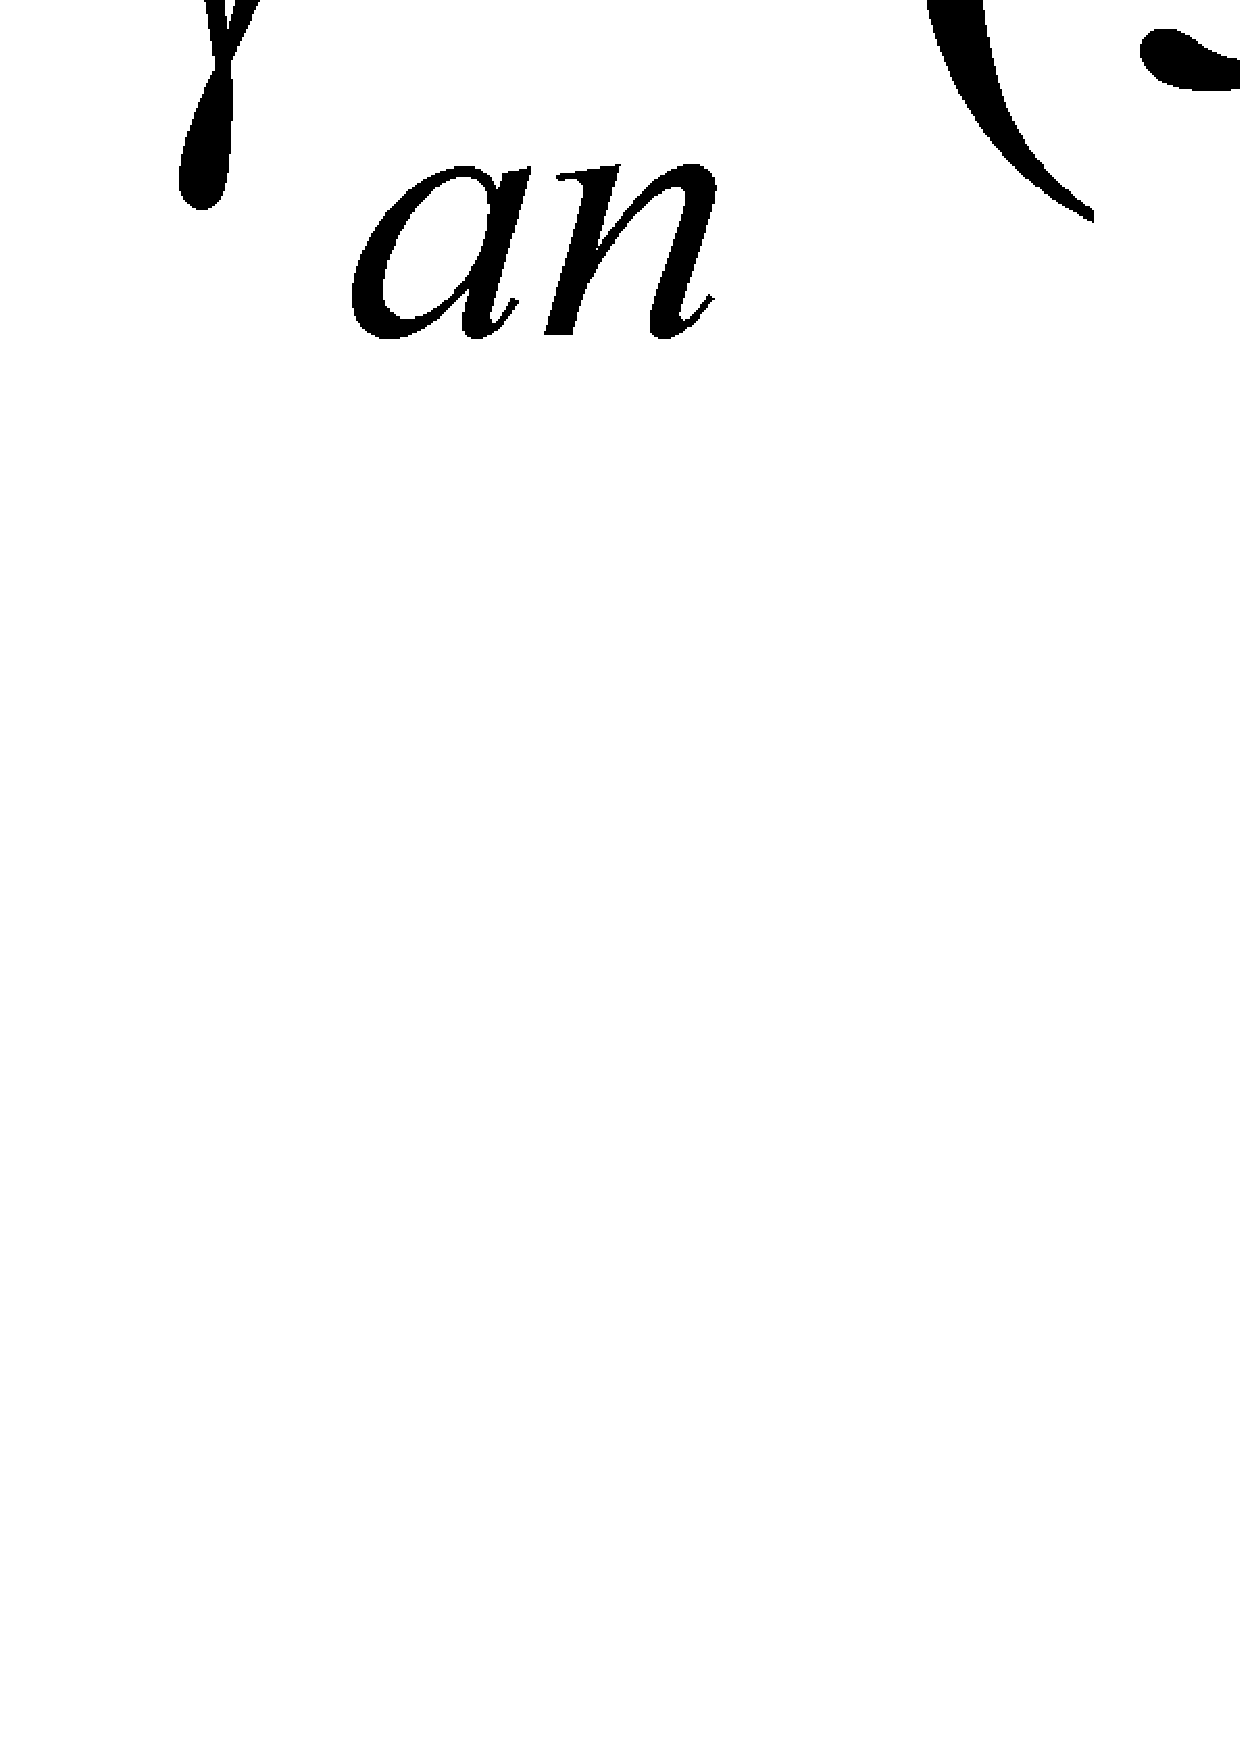
\includegraphics[width=0.7\textwidth]{Fig3_0}
\vspace{-3mm}
\caption{Схема, що ілюструє появу позитрону, позитрон--електронну анігіляцію
та емісію гамма-квантів.}
\vspace{-3mm}
\label{F30}
\end{figure}

Процеси, що відбуваються під час PAS при використанні ізотопного джерела, можна ілюструвати схемою,
зображеною на рис.~\ref{F30}.
Супутній до появи позитрона у джерелі процес емітування гамма кванта $\gamma_0$ може слугувати
відліком для вимірювання часу життя $\beta^+$--частинки.
Під час анігіляції з'являються два гамма кванти $\gamma_{an}$, енергія $E_\gamma$
та розподіл напряму руху яких залежать від стану електрону.
Наприклад, відхилення $\Delta\theta$ кута розльоту цих фотонів
від $180^\circ$ залежить від компоненти імпульсу електрону $p_\perp$, перпендикулярної до наступного
напрямку емісії:
\begin{equation}\label{PAStheta}
\Delta\theta=\frac{p_\perp}{m_0\,c}\,.
\end{equation}
В свою чергу, паралельна компонента імпульсу $p_\parallel$ викликає появу
так званого доплерівського зсуву $\Delta E_\gamma$ у енергії кожного з фотонів $E_\gamma$:
\begin{equation}\label{PASEgamma}
E_\gamma=m_0\,c^2\pm\Delta E_\gamma=m_0\,c^2\pm\frac{p_\parallel \,c}{2}\,,
\end{equation}
де
$m_0\,c^2=511$~кеВ --- енергія спокою електрону.
Рухаючись у кристалі,  позитрони швидко втрачають енергію внаслідок
іонізації атомів у вузлах кристалічної ґратки, збудженні електронів їхніх
внутрішніх оболонок (при високих кінетичних енергіях), генерації електронно-діркових пар та
фононному розсіянні (при низьких).
Цей процес термалізації займає лише декілька пікосекунд, що зазвичай набагато менше, ніж час життя позитронів.
Тому у виразах (\ref{PAStheta}) та (\ref{PASEgamma}) вважається, що визначальним
є саме імпульс електрону, оскільки позитрони перед анігіляцією мають низьку енергію.



Коефіцієнт поглинання позитронів можна оцінити за допомогою співвідношення \cite{PAS}
\begin{equation}
\alpha_+\approx\frac{\varrho\,\left[\text{г}/\text{см}^3\right]}{E_{+,m}^{1/4}\,[\text{МеВ}]}\:\text{см}^{-1}\,,
\end{equation}
де
$\varrho$ --- густина речовини,
$E_{+,m}$ --- максимальна енергія спектра позитронів (для $^{22}\text{Na}$ --- 0,54~МеВ).
Типові глибини проникнення ($\alpha^{-1}_+$) складають близько 110~мкм для Si та 40~мкм для GaN (при використання ізотопного джерела).

При розгляді позитронного опромінення використовують
таку величину як ймовірність поглинання (анігіляції) налітаючої частинки
при проходженні неї у речовині шляху одиничної довжини ($P_L$),
% $[P_L]=\text{см}^{-1}$).
розмірність якої обернено пропорційна відстані.
Залежність $P_L$ від глибини проникнення називається профілем поглинання (stopping profile).
При безпосередньому використанні радіоактивних джерел профіль екпоненційний:
\begin{equation}\label{PASPl1}
P_L(x)=\alpha_+\,\exp(-\alpha_+\,x)\,.
\end{equation}
Вираз (\ref{PASPl1}) записано у припущенні, що
напрям осі $X$ збігається з напрямом поширення позитронів,
а точка $x=0$ відповідає межі матеріалу.
Якщо взяти до уваги величини $\alpha_+$, то очевидно,
що такий режим опромінення придатний лише для дослідження об'ємних
(товщиною декілька сотень мікрометрів) матеріалів.
При характеризації дефектів у тонких плівках позитрони
бажано сповільнити до енергій менше 50~кеВ та, за можливості, монохроматизувати.
Зазвичай для сповільнення на поверхню джерела наносять тонкі плівки з матеріалу, що має
від'ємну роботу виходу для позитронів (вольфрам, твердотільні інертні гази), нанесені на поверхню джерела.
Для моноенергетичних позитронів профіль описується виразом
\begin{equation}\label{PASPl2}
P_L(x)=-\frac{d}{dx}\exp\left[-\left(\frac{x}{x_0}\right)^2\right]\,.
\end{equation}
де
$x_0$ --- розташування максимуму профілю поглинання.
При цьому середнє значення глибини проникнення $\bar{x}$  з одного боку
задовольняє умові $\bar{x}\simeq \,0,886\, x_0$ (профіль не симетричний),
а з другого --- визначається енергією позитрону $E_{+}$:
\begin{equation}
\bar{x}=\frac{4\cdot10^{-6}}{\varrho\left[\text{мкг}/\text{см}^3\right]}\cdot E_{+}^{1,6}\,[\text{кеВ}]\:\text{см}\,.
\end{equation}

У загальному випадку темп анігіляції позитронів $\lambda_+$ описується виразом
\begin{equation}\label{PASL}
\lambda_+=\frac{1}{\tau_+}=\pi\,r_e^2\,c\int\gamma_+(\overrightarrow{r})\left|\psi_+(\overrightarrow{r})\right|^2\,\rho_e(\overrightarrow{r})\,d\overrightarrow{r}\,.
\end{equation}
де
$\tau_+$ --- час життя позитронів,
$r_e=\frac{q^2}{4\pi\varepsilon_0 m c^2}\approx2,8\cdot10^{-15}\,\text{м}$ --- класичний радіус електрону,
$\psi_+$ --- хвильова функція позитрону,
$\rho_e$ --- електронна густина,
$\gamma_+(\overrightarrow{r})$ --- так званий фактор підсилення, багаточастинковий ефект,
який враховує екранування позитронів електронами і визначається величиною
кореляційної функції електрон--позитронної пари при нульовій відстані \cite{tuomisto2019}.
Як видно з (\ref{PASL}), $\lambda_+$ пропорційна перекриттю позитронних та електронних густин.

Позитрони, як і електрони, можуть локалізуватися біля порушень ґратки --- тобто, знаходячись в околі дефектів мати енергію,
яка є недозволеною для них у ідеальній ґратці.
При цьому
\begin{enumerate}[label=\asbuk*),leftmargin=0em,itemindent=1.5em]
%\begin{enumerate}[label=\arabic*),leftmargin=0em,itemindent=1.5em]
\item для дефектів вакансійного типу відповідні рівні глибокі, енергія іонізації $E_{t+}\geq$1~еВ;
\item для від'ємно заряджених домішок заміщення та міжвузольних дефектів рівні мілкі,
 енергія зв'язку становить $(10\div100)$~меВ і
непогано описується у наближенні теорії ефективної маси.
%енергія зв'язку становить $10\div100$~меВ, а отже при температурі $100\div300$~К відповідні стані іонізовані.
\end{enumerate}

Швидкість захоплення позитронів дефектом описується виразом
\begin{equation}\label{PASc}
c_+=\frac{N_t\,\mu_t}{\rho_N}\,.
\end{equation}
де
$\rho_N$ --- концентрація ядер,
а коефіцієнт $\mu_t$ залежить як від типу дефекту, так і від властивостей основної ґратки.

Для додатно заряджених як вакансій, так і дефектів іншого типу, значення $\mu_t$
настільки малі, що за час життя позитрону відповідні процеси практично не встигають відбуватися і тому
PAS не здатна виявляти дефекту у такому зарядженому стані.
Для нейтральної вакансії $\mu_t\approx10^{14}\div10^{15}$~c$^{-1}$ і практично не залежить від температури;
для негативно зарядженої $\mu_t\approx10^{15}\div10^{16}$~c$^{-1}$ при $T=300$~K і зростає при
зниженні температури (у спрощеному випаду при врахуванні лише зміни теплової швидкості
позитрону $\mu_t\sim T^{-1/2}$).
Для дефектів, пов'язаних з негативно зарядженими іонами величина $\mu_t$ приблизно така ж сама
як для V$^-$.
Проте необхідно врахувати, що відповідно до принципу детальної рівноваги
\begin{equation}\label{PASce}
\frac{e_+}{c_+}=\frac{1}{N_t}\left(\frac{m_+^*kT}{2\pi\hbar^2}\right)^{3/2}\exp\left(-\frac{E_{t+}}{kT}\right)\,,
\end{equation}
де
$e_+$ --- швидкість емісії позитронів,
$m_+^*$ --- ефективна маса позитрону, зазвичай $m_+^*\approx1,5 m_0$.
А отже, для мілких рівнів анігіляція захоплених позитронів може спостерігатися лише при
$T<100$~К, при вищих температурах вони термічно іонізовані.
В той же час для вакансій $e_+\approx0$.

Припустимо, що
$p_{b}^+(t)$ --- частка вільних позитронів у кристалі в момент часу $t$ відносно до загальної початкової кількості позитронів, а
$p_{t,j}^+(t)$  --- частка позитронів, захоплених дефектами $j$--го типу.
Тоді систему рівнянь, яка описує кінетику зміни кількості позитронів можна записати у вигляді
\begin{equation}\label{PASdin}
\left\{
\begin{aligned}%{rl}
\frac{dp_{b}^+(t)}{dt}=& -\lambda_{+,b} \:p_{b}^+ - \sum_j c_{+,j} \:p_{b}^+ + \sum_j e_{+,j} \,p_{t,j}^+ \,,\\
\frac{dp_{t,j}^+(t)}{dt}=& c_{+,j} \:p_{b}^+ - \lambda_{+,tj}\,p_{t,j}^+ - e_{+,j} \,p_{t,j}^+ \,,
\end{aligned} \right.
\end{equation}
де
$\lambda_{+,b}$ та $\lambda_{+,tj}$ описують темп анігіляції позитронів, які знаходяться
у об'ємі кристалу та які захоплені дефектом $j$--го  типу.
Вважається, що у початковий момент часу $p_{b}^+(0)=1$, $p_{t,j}^+(0)=0$ --- всі позитрони вільні.

Наприклад, якщо у кристалі присутні один дефект вакансійного типу
(характеризується параметрами $\lambda_{+,\mathrm{V}}$, $c_{+,\mathrm{V}}$ та $e_{+,\mathrm{V}}\approx0$)
та один дефект, що є причиною появи мілкого позитронного рівня з параметрами
$\lambda_{+,\mathrm{ST}}$, $c_{+,\mathrm{ST}}$ та $e_{+,\mathrm{ST}}$ (<<ST>> --- shallow trap),
то система рівнянь виглядатиме наступним чином
\begin{equation}\label{PASdin2}
\left\{
\begin{aligned}%{rl}
\frac{dp_{b}^+}{dt}=& -(\lambda_{+,b}+c_{+,\mathrm{V}}+c_{+,\mathrm{ST}}) \:p_{b}^+ +e_{+,\mathrm{ST}}\,p_{\mathrm{ST}}^+ \,,\\
\frac{dp_{\mathrm{V}}^+}{dt}=& c_{+,\mathrm{V}} \:p_{b}^+ - \lambda_{+,\mathrm{V}}\,p_{\mathrm{V}}^+ \,,\\
\frac{dp_{\mathrm{ST}}^+}{dt}=& c_{+,\mathrm{ST}} \:p_{b}^+ - (\lambda_{+,\mathrm{ST}}+e_{+,\mathrm{ST}})\,p_{\mathrm{ST}}^+ \,.
\end{aligned} \right.\tag{\ref{PASdin}\,$'$}
\end{equation}
Сумарна частка електронів, які ще не проанігілювали у момент часу $t$
(ймовірність, що позитрон у цей момент часу ще існує) описується виразом
\begin{equation}\label{PASn1}
p^+(t)=dp_{b}^+(t) + p_{\mathrm{V}}^+(t) + p_{\mathrm{ST}}^+(t)\,.
\end{equation}
Після розв'язання системи рівнянь (\ref{PASdin2}) вираз (\ref{PASn1})  можна
переписати у вигляді
\begin{equation}\label{PASn2}
p^+(t)=\sum_{i=1}^3I_i\exp\left(-\frac{t}{\tau_i}\right)\,,\tag{\ref{PASn1}\,$'$}
\end{equation}
де
$I_i$ та $\tau_i$ будуть залежать від $\{\lambda_{+,b},\lambda_{+,\mathrm{V}},\lambda_{+,\mathrm{ST}},c_{+,\mathrm{V}},c_{+,\mathrm{ST}},e_{+,\mathrm{ST}}\}$,
а також $\sum I_i=1$.

Взагалі, у PAS існує два основних підходи до визначення стану дефектів ---позитронна спектроскопія часу життя
та спектроскопія доплерівського уширення.
Розглянемо їх детальніше.

\section{Позитронна спектроскопія часу життя}\label{secPAS_PSLT}
У цьому варіанті PAS дослідження зазвичай проводять з використанням ізотопного натрієвого джерела,
причому воно використовується у формі NaCl і зберігається у вигляді водного розчину.
У експерименті джерело розміщується між двома ідентичними зразками
(утворюється сандвіч--подібна структура) і
вимірюється проміжок часу між двома подіями:
\begin{itemize}[leftmargin=0em,itemindent=1.5em]
\item появою $\gamma$--фотона з енергією 1,2745~МеВ, що є свідченням появи позитрона і відповідає переходу ізотопу неону зі збудженого стану;
\item появою фотона (або двох) з енергією 0,511~МеВ, яка пов'язана з анігіляцією.
\end{itemize}

\begin{figure}[b]
\center
\vspace{-2mm}
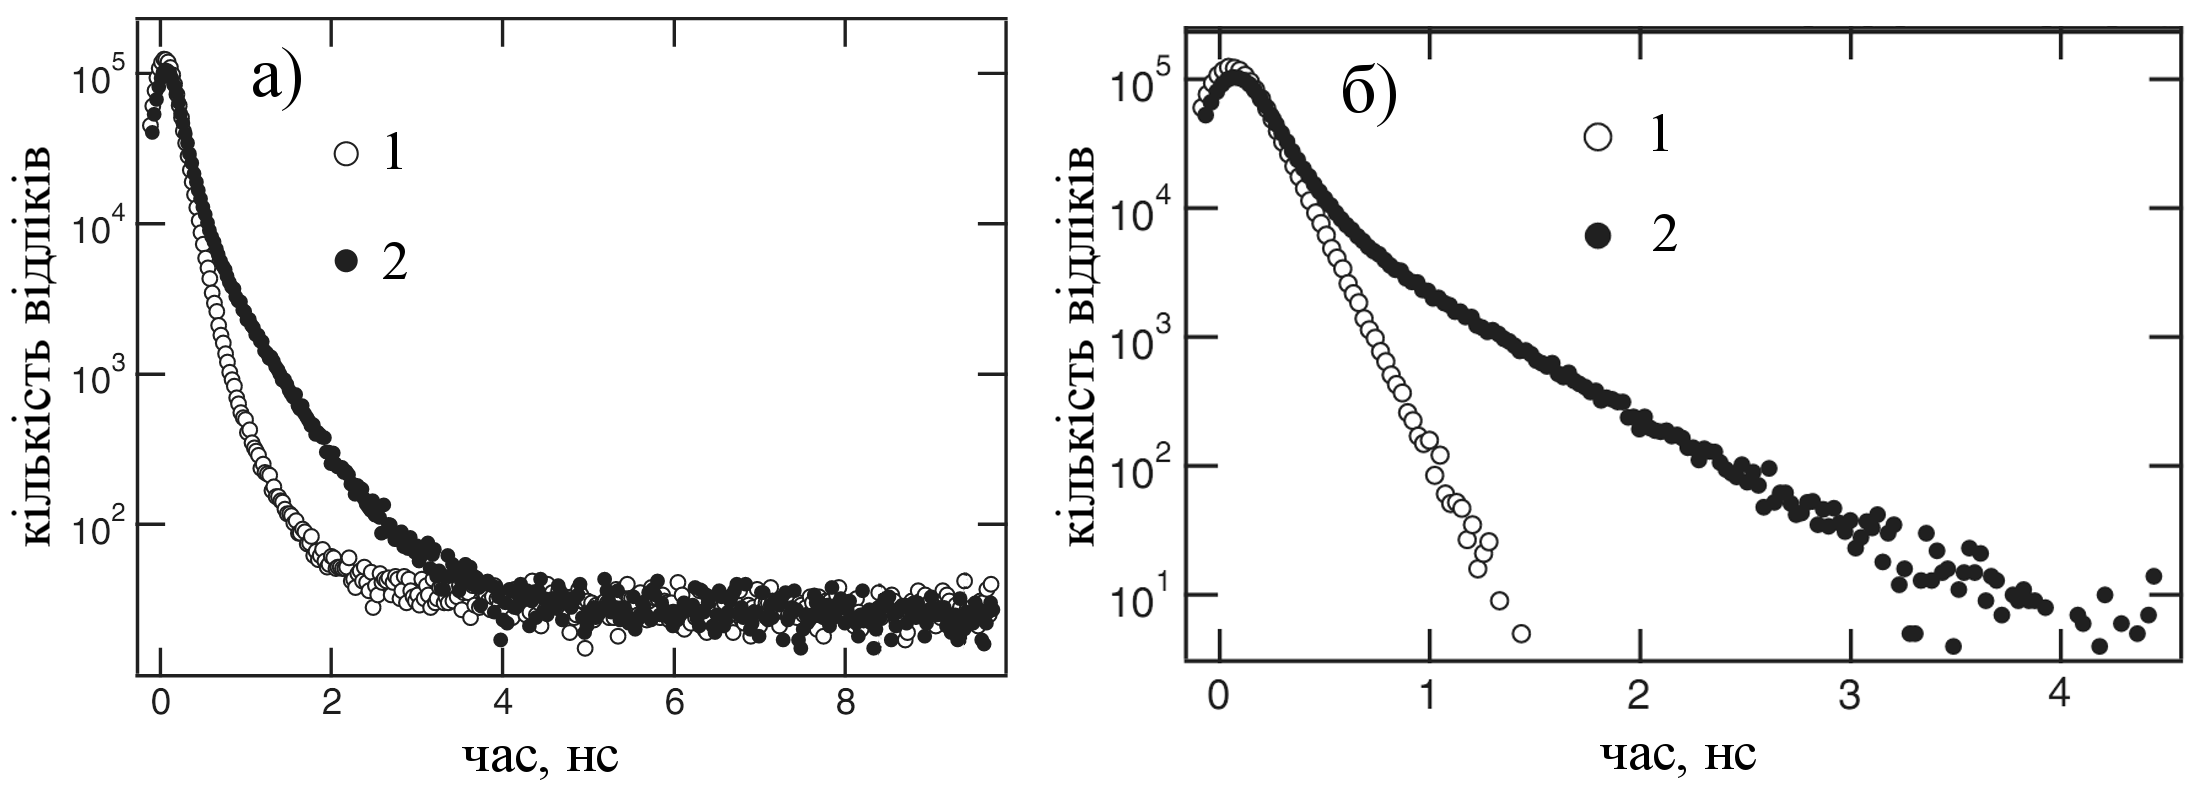
\includegraphics[width=0.97\textwidth]{Fig3_1}
\vspace{-3mm}
\caption{Спектр часу життя позитронів у випадку наявності однієї анігіляційної компоненти
(криві 1) і двох (2) до (частина а) та після (б) врахування фону та
анігіляції у джерелі.
Рисунок адаптовано з \cite{PAS}.}
\vspace{-3mm}
\label{F31}
\end{figure}

У даному випадку спектром є гістограма кількості анігіляційних подій залежно від проміжку часу.
Приклад відповідної залежності наведено на рис.~\ref{F31},а.
Після реєстрації враховується наявність фонового шуму та анігіляцію у джерелі --- рис.~\ref{F31},б.
Надалі визначається кількість компонент у спадній ділянці.
У найпростішому випадку це можна зробити за кількістю лінійних ділянок на логарифмічній залежності
кількості подій від часу.
Наприклад, для кривої 1 на рис.~\ref{F31},б. спостерігається одна така ділянка,
для кривої 2 --- дві.
Після цього отримані дані апроксимуються виразом, подібним (\ref{PASn2}) і визначаються параметри $\{I_i\}$ та $\{\tau_i\}$.
Зокрема, для кривої 2 має бути використана формула
\begin{equation*}
p^+(t)=I_1\exp\left(-\frac{t}{\tau_1}\right)+I_2\exp\left(-\frac{t}{\tau_2}\right)\,,
\end{equation*}
і визначені величини $I_1$, $I_2$, $\tau_1$ та $\tau_2$.
У загальному випадку кількість доданків у сумі теж є параметром апроксимації.

Зв'язок визначених величин з параметрами дефектів залежить від можливих шляхів анігіляції позитронів.
Наприклад, криві 2 на рис.~\ref{F31} свідчить про два можливих механізми зникнення позитронів --- при зустрічі з електронами
у недеформованій ґратці та поблизу дефектів вакансійного типу і
тому рівняння, що описують кінетику анігіляції, виглядатимуть наступним чином:
\begin{gather}
 \frac{dp_{b}^+(t)}{dt}= -\lambda_{+,b}\:p_{b}^+ - c_{+,\mathrm{V}} \:p_{b}^+ \,, \label{PASnb1}\\
\frac{dp_{\mathrm{V}}^+(t)}{dt}= - \lambda_{+,\mathrm{V}}\,p_{\mathrm{V}}^+ + c_{+,\mathrm{V}} \:p_{b}^+ \,.\label{PASnv1}
\end{gather}
Якщо б компонент у спадній ділянці було б більше, то система рівнянь мала б бути складнішою,
але в нашому ілюстративному випадку обмежимося лише наявністю одного вакансійного дефекту.
Тим паче, що на практиці така ситуація спостерігається доволі часто.

У рівнянні (\ref{PASnb1}) змінні розділяються і тому його розв'язок отримати досить просто
\begin{equation}\label{PASnb2}
p_{b}^+(t)=p_{b}^+(0)\exp\left[-(\lambda_{+,b}+c_{+,\mathrm{V}})\,t\,\right]=\exp\left(-\frac{t}{\tau_1}\right)\,,
\end{equation}
тобто $\tau_1^{-1}=\lambda_{+,b}+c_{+,\mathrm{V}}=\tau_{+,b}^{-1}+c_{+,\mathrm{V}}$,
де $\tau_{+,b}$ --- час життя позитронів у ідеальній ґратці.
У виразі (\ref{PASnb2}) враховано, що в початковий момент часу всі позитрони вільні.
Отже, рівняння зміни кількості захоплених дефектом позитронів неоднорідне
\begin{equation}\label{PASnv2}
\frac{dp_{\mathrm{V}}^+(t)}{dt}+\lambda_{+,\mathrm{V}}\,p_{\mathrm{V}}^+=c_{+,\mathrm{V}}\:\exp\left(-\frac{t}{\tau_1}\right)\,.
\end{equation}
Розв'язок однорідного рівняння має вигляд
\begin{equation}
p_{\mathrm{V},\mbox{одн}}^+(t)=p_{\mathrm{V}0}^+\exp\left(-\lambda_{+,\mathrm{V}}\,t\right)
  =p_{\mathrm{V}0}^+\:\exp\left(-\frac{t}{\tau_2}\right)\,,
\end{equation}
де $\tau_2=\lambda_{+,\mathrm{V}}^{-1}=\tau_{+,\mathrm{V}}$ --- час життя позитрону в околі вакансійного дефекту.
Частковий розв'язок неоднорідного рівняння шукатимемо у вигляді
\begin{equation}
p_{\mathrm{V},\mbox{неодн}}^+(t)=A\exp\left(-\frac{t}{\tau_1}\right)\,,
\end{equation}
де величину константи $A$ можна отримати шляхом підстановки останнього виразу у (\ref{PASnv2}):
\begin{gather*}
-\frac{A}{\tau_1}\exp\left(-\frac{t}{\tau_1}\right)+\lambda_{+,\mathrm{V}}A\exp\left(-\frac{t}{\tau_1}\right)=c_{+,\mathrm{V}}\:\exp\left(-\frac{t}{\tau_1}\right)\,,\\
A=\frac{c_{+,\mathrm{V}}}{\lambda_{+,\mathrm{V}}-\tau_1^{-1}}= \frac{c_{+,\mathrm{V}}}{\tau_{+,\mathrm{V}}^{-1}-\tau_{+,b}^{-1}-c_{+,\mathrm{V}}}
=\frac{c_{+,\mathrm{V}}}{\tau_2^{-1}-\tau_1^{-1}}\,.
\end{gather*}
Тобто загальний розв'язок має вигляд
\begin{equation}\label{PASnb3}
p_{\mathrm{V}}^+(t)=p_{\mathrm{V}0}^+\:\exp\left(-\frac{t}{\tau_2}\right)+\frac{c_{+,\mathrm{V}}}{\tau_2^{-1}-\tau_1^{-1}}\exp\left(-\frac{t}{\tau_1}\right)\,.
\end{equation}
Враховуючи,
що $p_{\mathrm{V}}^+(0)=0$, отримуємо
\begin{equation}\label{PASnb4}
p_{\mathrm{V}0}^+=\frac{c_{+,\mathrm{V}}}{\tau_1^{-1}-\tau_2^{-1}}\,.
\end{equation}
Взявши до уваги вирази (\ref{PASnv2}), (\ref{PASnb3}) та (\ref{PASnb4}),
загальний вираз для кінетики зміни кількості позитронів може бути записаний у вигляді
\begin{equation}\label{PASnRez}
p_{b}^+(t)
%=p_{b}^+(t)+p_{\mathrm{V}}^+(t)
=\exp\left(-\frac{t}{\tau_1}\right)
         +\frac{c_{+,\mathrm{V}}}{\tau_1^{-1}-\tau_2^{-1}}\left[\exp\left(-\frac{t}{\tau_2}\right)-\exp\left(-\frac{t}{\tau_1}\right)\right]\,.
\end{equation}
Відповідно, система співвідношень між експериментально визначеними параметрами
та характеристиками позитронної анігіляції буде наступною
\begin{equation}\label{PASsist}
\left\{
\begin{aligned}
 I_2=&  \,\frac{c_{+,\mathrm{V}}}{c_{+,\mathrm{V}}-\lambda_{+,\mathrm{V}}+\lambda_{+,b}}\,,\\
I_1=& \,1-I_2 \,,\\
\tau_2=&\,\lambda_{+,\mathrm{V}}^{-1}=\tau_{+,\mathrm{V}}\,,\\
\tau_1=&\,(\lambda_{+,b}+c_{+,\mathrm{V}})^{-1}=(\tau_{+,b}^{-1}+c_{+,\mathrm{V}})^{-1}\,.
\end{aligned} \right.
\end{equation}

Для визначення величини $\lambda_{+,b}=\tau_{+,b}^{-1}$ можна використати
опорний зразок з того самого матеріалу, але відсутнє вакансійне захоплення і сигнал складається лише з однієї
експоненційної компоненти.
Зауважимо, що $\tau_{+,b}$ слабко залежить від рівня легування напівпровідника і може слугувати
табличною характеристикою матеріалу.
Наприклад, для кремнію $\tau_{+,b}\approx221$~пс.
Щодо $\tau_{+,\mathrm{V}}$, то ця величина залежить від атомної конфігурації дефекту та дозволяє ідентифікувати його тип ---
наприклад у Таблиці~\ref{tabltau} приведені значення для  вакансійних комплексів різного розміру
у кремнії.


\begin{table}[bth]
\caption {Час життя позитронів в околі вакансійних кластерів у кремнії}
\label{tabltau} %\center{
\vspace{-3mm}
%\begin{tabular}{|p{0.18\textwidth}|*{5}{p{0.14\textwidth}|}}
\begin{tabularx}{\textwidth}{|>{\centering\arraybackslash}X|>{\centering\arraybackslash}X|>{\centering\arraybackslash}X|>{\centering\arraybackslash}X|>{\centering\arraybackslash}X|>{\centering\arraybackslash}X|}
  \hline
  дефект & V&V$_2$ &V$_3$&V$_4$&V$_5$    \tabularnewline \hline
  $\tau_{+,\mathrm{V}}$, пс & 254&299&321&330&355   \tabularnewline \hline
\end{tabularx}
%\end{tabular}
%}
\end{table}

Використовуючи  величину $c_{+,\mathrm{V}}$ та теоретичну розраховане значення $\mu_\mathrm{V}$
можна оцінити концентрацію вакансій -- див. вираз (\ref{PASc}).


В позитронній спектроскопії часу життя можна також розглядати
парціальні анігіляції в різних станах $\eta_+$.
Наприклад,
для системи з двома механізмами анігіляції
розглядати $\eta_{+,b}$ та $\eta_{+,\mathrm{V}}$ ---
частки позитронів, які анігілювали у ґратці та в околі вакансійних
дефектів, відповідно;
у більш загальному випадку говорити про $\eta_{+,b}$ та $\{\eta_{+,tj}\}$.
Зауважимо, що $\eta_{+,b}+\eta_{+,\mathrm{V}}=1$
(або $\eta_{+,b}+\sum_j\eta_{+,tj}=1$).
Тоді середній час життя позитронів $\left\langle\tau_+\right\rangle$
з одного боку буде визначати виразом
\begin{equation*}
\left\langle\tau_+\right\rangle=\int_0^\infty t\left(-\frac{dp^+(t)}{dt}\right)dt=I_1\tau_{1}+I_2\tau_{2}\,;
\quad\left(\text{або}\,\left\langle\tau_+\right\rangle=\sum I_i \tau_{i}\right)\,,
\end{equation*}
а з іншого
\begin{equation*}
\left\langle\tau_+\right\rangle=\eta_{+,b}\tau_{+,b}+\eta_{+,\mathrm{V}}\tau_{+,\mathrm{V}}\,;
\quad\left(\text{або}\,\left\langle\tau_+\right\rangle=\eta_{+,b}\tau_{+,b}+\sum \eta_{+,tj}\tau_{+,tj}\right)\,.
\end{equation*}
Нагадаємо, що кількість доданків у сумі першого виразу (по компонентам спадної залежності) на
одиницю більша ніж кількість доданків у сумі другого виразу (по типам активних дефектів).
З цього, зокрема, випливає, що
\begin{gather*}
\eta_{+,b}=\frac{\lambda_{+,b}}{\lambda_{+,b}+c_{+,\mathrm{V}}}\,;\quad
\eta_{+,\mathrm{V}}=\frac{c_{+,\mathrm{V}}}{\lambda_{+,b}+c_{+,\mathrm{V}}} \\
\left(\eta_{+,b}=\frac{\lambda_{+,b}}{\lambda_{+,b}+\sum c_{+,tj}}\,;\quad
\eta_{+,tl}=\frac{c_{+,tl}}{\lambda_{+,b}+\sum c_{+,tj}} \right)\,.
\end{gather*}

$\left\langle\tau_+\right\rangle$ взагалі може бути ключовим параметром,
який безпосередньо визначається з експериментальних залежностей.
Наприклад, коефіцієнт захоплення позитронів дефектом можна визначити саме через цю величину
\begin{equation*}
c_{+,\mathrm{V}}=\frac{1}{\tau_{+,b}}\,\cdot\,\frac{\left\langle\tau_+\right\rangle-\tau_{+,b}}{\tau_{+,\mathrm{V}}-\left\langle\tau_+\right\rangle}\,.
\end{equation*}


\begin{figure}[!b]
\center
\vspace{-5mm}

\includegraphics[width=0.6\textwidth]{Fig3_2}
\vspace{-3mm}
\caption{Схематичні температурні
залежності рівня Фермі (а),
амплітуди компоненти спектра PAS (б),
часу життя позитронів в околі вакансії (в)
та середнього часу життя позитронів (г).
В температурній області $I$ вакансія переважно
перебуває у однократно від'ємно зарядженому стані,
в області $II$ --- в нейтральному.
}
\vspace{-3mm}
\label{F32}
\end{figure}

Якщо проводити вимірювання при різних температурах, то
за відсутністю (чи наявністю) температурної залежності $c_{+,\mathrm{V}}$ можна зробити
висновок про нейтральність (чи негативний заряд) вакансійного дефекту;
Крім того, як вже зазначалося вище, величини $\tau_{+,\mathrm{V}}$ та $c_{+,\mathrm{V}}$ залежать від зарядового стану
вакансії, який, в свою чергу, визначається положенням рівня Фермі, що теж змінюється з температурою.
Наприклад, для напівпровідника з електронною провідністю
\begin{equation}\label{EF}
E_F(T)=\frac{1}{2}(E_D+E_C)-\frac{1}{2}kT\ln\left(\frac{N_C(T)}{\gamma_{g,D}N_D}\right)\,,
\end{equation}
де
$E_D$ --- енергетичний рівень, пов'язаний з донорною домішкою,
$\gamma_{g,D}$ --- фактор його виродження.
Якщо положення рівня вакансії $E_{t}$ таке, що
в досліджуваному температурному діапазоні змінюється його розташування
відносно $E_F$, то на температурних залежностях $\tau_{+,\mathrm{V}}$ (або $\tau_2$),
$c_{+,\mathrm{V}}$ (або $I_2$) та $\left\langle\tau_+\right\rangle$
має спостерігатися певний стрибок --- див. рис.~\ref{F32}, намальований для випадку рівня  $E_t(0/-)$.
При цьому розташування стрибка ($T_{h}$) дозволяє визначити розташування рівня дефекту
\begin{equation}
E_t =E_F(T_{h})\,.
\end{equation}

Таким чином, позитронна спектроскопія часу життя дозволяє визначити наявність вакансій,
їхній зарядовий стан, концентрацію, розмір кластерів та, при вимірюваннях у певному температурному діапазоні,
положення енергетичного рівня.
Змінюючи енергію позитронів, можна проводити аналіз дефектів по глибині зразка.
Інформацію про негативнозаряджені іони, зокрема їхню концентрацію,
можна отримати у випадку, коли вони конкурують з вакансіями у захоплення позитронів і таким чином впливають на середній час життя позитронів.

\section{Спектроскопія доплерівського уширеня}\label{secPAS_SDU}

В цьому випадку вимірюється енергетична ширина лінії фотону,
який виник при анігіляції --- див. рис.~\ref{F34},а.
Уширення лінії пов'язане з наявністю у анігілюючого електрону імпульсу,
а отже в результаті взаємодії позитрону з квазі--вільним електроном, енергія якого відповідає
зоні провідності, та зі зв'язаним електроном у валентній зоні
з'являються $\gamma$--кванти з суттєво різним відхиленням енергії від $m_0c^2$
--- див. вираз (\ref{PASEgamma}).

\begin{figure}[!t]
\center
\vspace{-5mm}
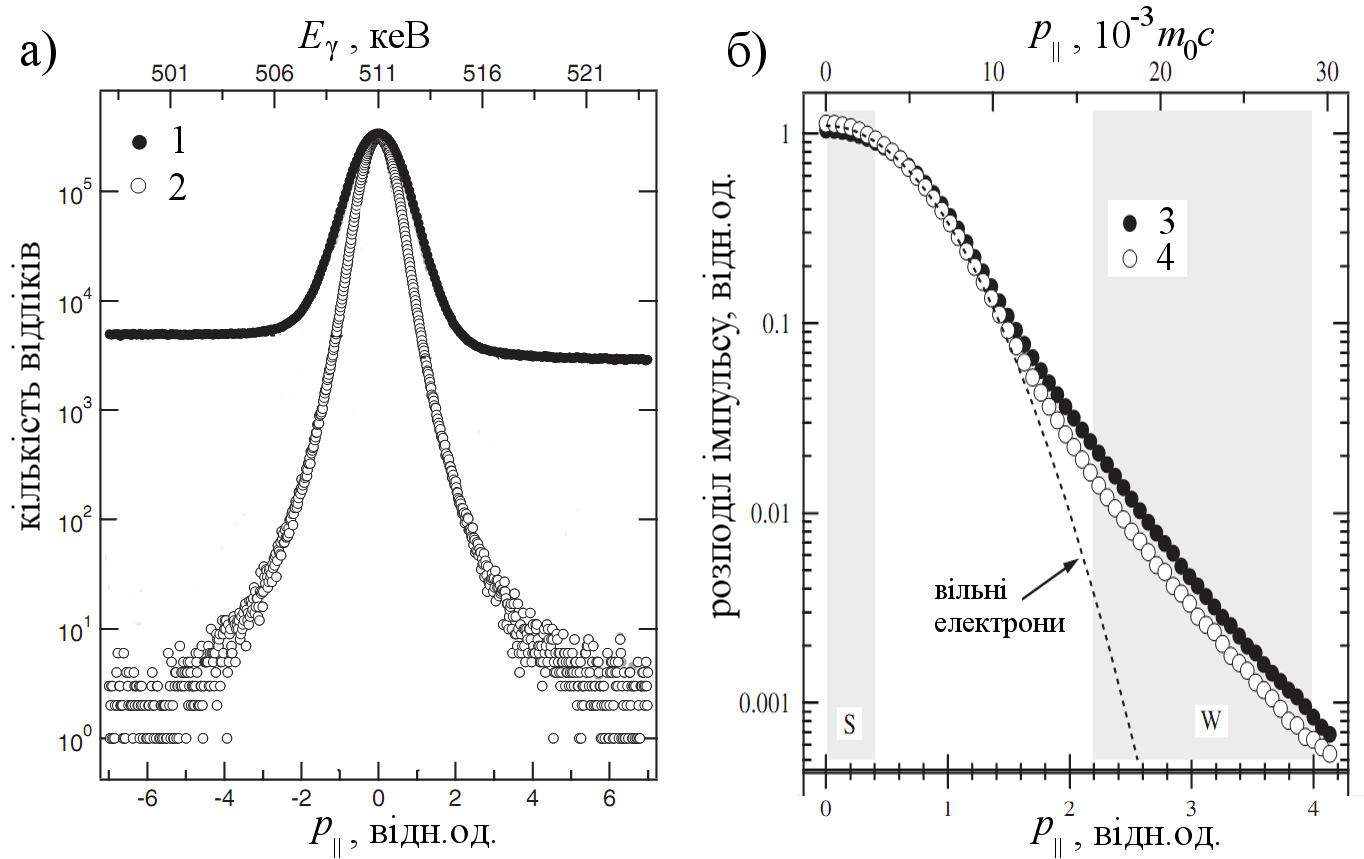
\includegraphics[width=0.95\textwidth]{Fig3_4}
\vspace{-3mm}
\caption{(а) Спектр доплерівського уширення,
отриманий за допомогою одного (крива 1) та двох (2)
детекторів.
(б) Нормований розподіл імпульсу електронів
по модулю його значення для ґратки GaN (3)
та вакансії галію (4).
Пунктиром показано розподіл для вільних електронів.
Рисунок адаптовано з \cite{PAS}.
}
\vspace{-3mm}
\label{F34}
\end{figure}

Позитрони мають бути сповільнені, зазвичай до енергій $0,1\div50$~кеВ.
Для підвищення відношення сигнал--шум, тобто для того щоб реєструвати лише фотони, пов'язані з анігіляцією,
найчастіше використовуються два колінеарно розташовані детектори.
В цьому випадку, подією, яка береться до уваги, є поява двох $\gamma$--квантів, які
а)~рухаються у приблизно протилежних напрямках;
б)~з'явилися одночасно;
в)~мають загальну енергію близько $1,022$~МеВ.
Загальна кількість подій, що реєструються у одному експерименті,
зазвичай перевищує $10^6$.

\begin{figure}[!b]
\center
\vspace{-5mm}
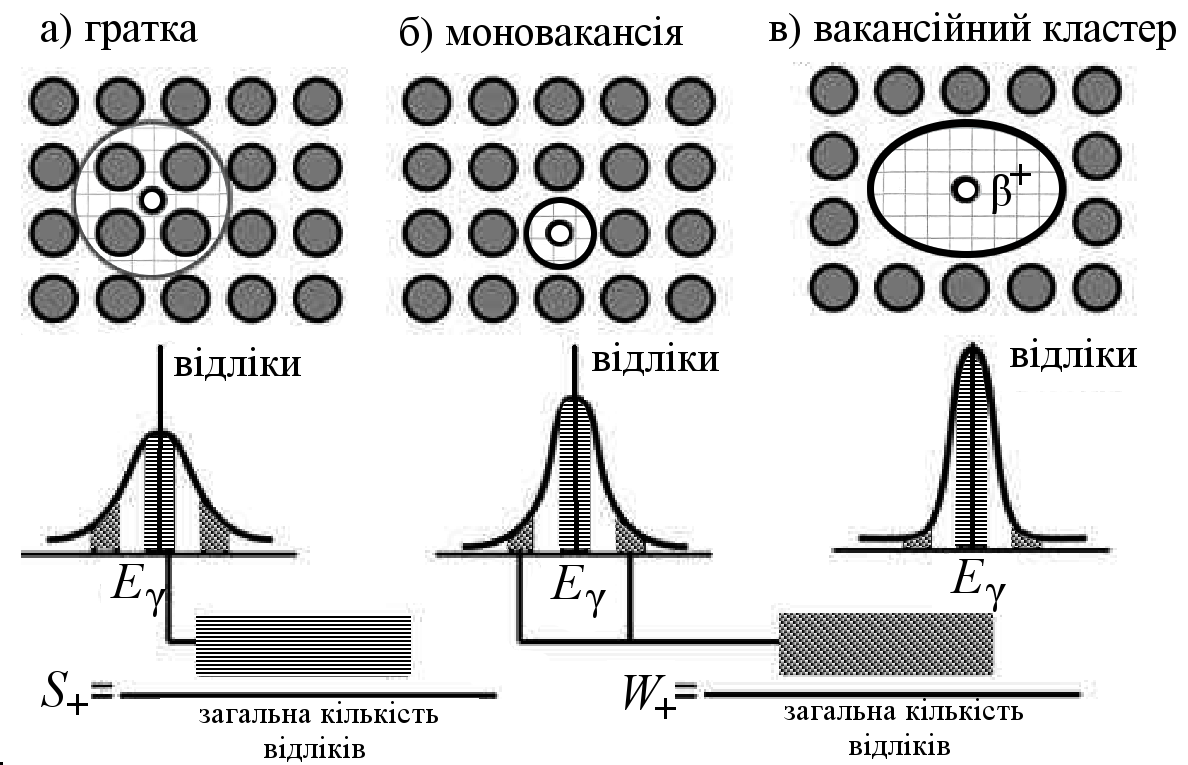
\includegraphics[width=0.75\textwidth]{Fig3_5}
\vspace{-3mm}
\caption{Схема доплерівського спектра при анігіляції
позитронів у делокалізованому стані (а) та захоплених вакансією (б) чи вакансійним кластером (в).
Рисунок адаптовано з \cite{Uedono_2014}.
}
\vspace{-3mm}
\label{F35}
\end{figure}

За отриманою залежністю визначають так звані низько--імпульсний параметр форми
(low--momentum shape parameter) $S_+$ (як відношення кількості подій в центральній частині
анігіляційної лінії до загальної кількості подій та
та високо--імпульсний параметр (high--momentum shape parameter) $W_+$ (як частка подій у бічній області).
Інша назва $S_+$ та $W_+$ --- valence and core annihilation parameters, відповідно.
На рис.~\ref{F34},б та \ref{F35} показано типові області, які вибираються для обчислення $S_+$ та $W_+$.
На практиці, ці регіони вибираються таким чином, що $S_+\approx0,5$,
а нижні границі симетричних відносно піку областей для визначення $W_+$ знаходяться достатньо далеко від
максимуму, щоб мінімізувати вплив енергетичного розподілу вільних електронів.

При анігіляції у бездефектній області кристалу та в околі вакансійного дефекту
величини вказаних параметрів
відрізняються внаслідок відмінностей у відносних кількостях електронів внутрішніх
та зовнішніх оболонок --- див. рис.~\ref{F34},б та \ref{F35}.
Тому, наприклад для простого випадку, який розглядався у попередньому параграфі,
має виконуватися:
\begin{equation*}
S_+=\eta_{+,b}+\eta_{+,\mathrm{V}}S_{+,\mathrm{V}}\,;\qquad
W_+=\eta_{+,b}W_{+,b}+\eta_{+,\mathrm{V}}W_{+,\mathrm{V}}\,,
\end{equation*}
або для більш загального
\begin{equation*}
S_+=\eta_{+,b}+\sum_j\eta_{+,tj}S_{+,tj}\,;\qquad
W_+=\eta_{+,b}W_{+,b}+\sum_j\eta_{+,tj}W_{+,tj}\,.
\end{equation*}

Як наслідок, знаючи низько--імпульсний параметр форми ідеального кристалу $S_{+,b}$
та низько--імпульсний параметр форми вакансії $S_{+,\mathrm{V}}$
спираючись на визначене значення $S_+$ можна було б оцінити
концентрацію дефектів.
Проте реально абсолютні значення $S_+$ та $W_+$ суттєво залежать
від геометрії детекторів, їхньої роздільної здатності, калібрування
вимірювальної системи, коефіцієнта підсилення підсилювача,
напрямку вимірів тощо і тому фактично не мають змісту.
Для оцінки концентрацій використовуються зазвичай
значення $S_+$ та $W_+$, нормовані до $S_{+,b}$ та $W_{+,b}$,
отримані в цій же самій експериментальній  конфігурації
для опорного бездефектного зразка.
Також можна оцінювати еволюцію дефектного складу одного й того ж зразка внаслідок
певних зовнішніх впливів.
Перезарядка дефекту викликає зміни, насамперед, у величині параметра $S_+$.
Тому за розташуванням стрибка на температурній залежності
цієї величина можна зробити висновок
про енергетичне розташування відповідного рівня,
подібно до того як це описано раніше.



Важливим у цьому методі є те, що $W_+$ містить
інформацію про хімічні елементи (атоми), які знаходяться біля місця анігіляції.
Теоретично можливо розрахувати форму анігіляційної лінії для
різних комплексів --- див. приклади на рис.~\ref{F36}.
Порівнюючи розрахунки з експериментально отриманими значеннями
(насамперед беруть до уваги величини $S_+/W_+$) проводять
визначення типів дефектів.

\begin{figure}[!b]
\center
\vspace{-5mm}
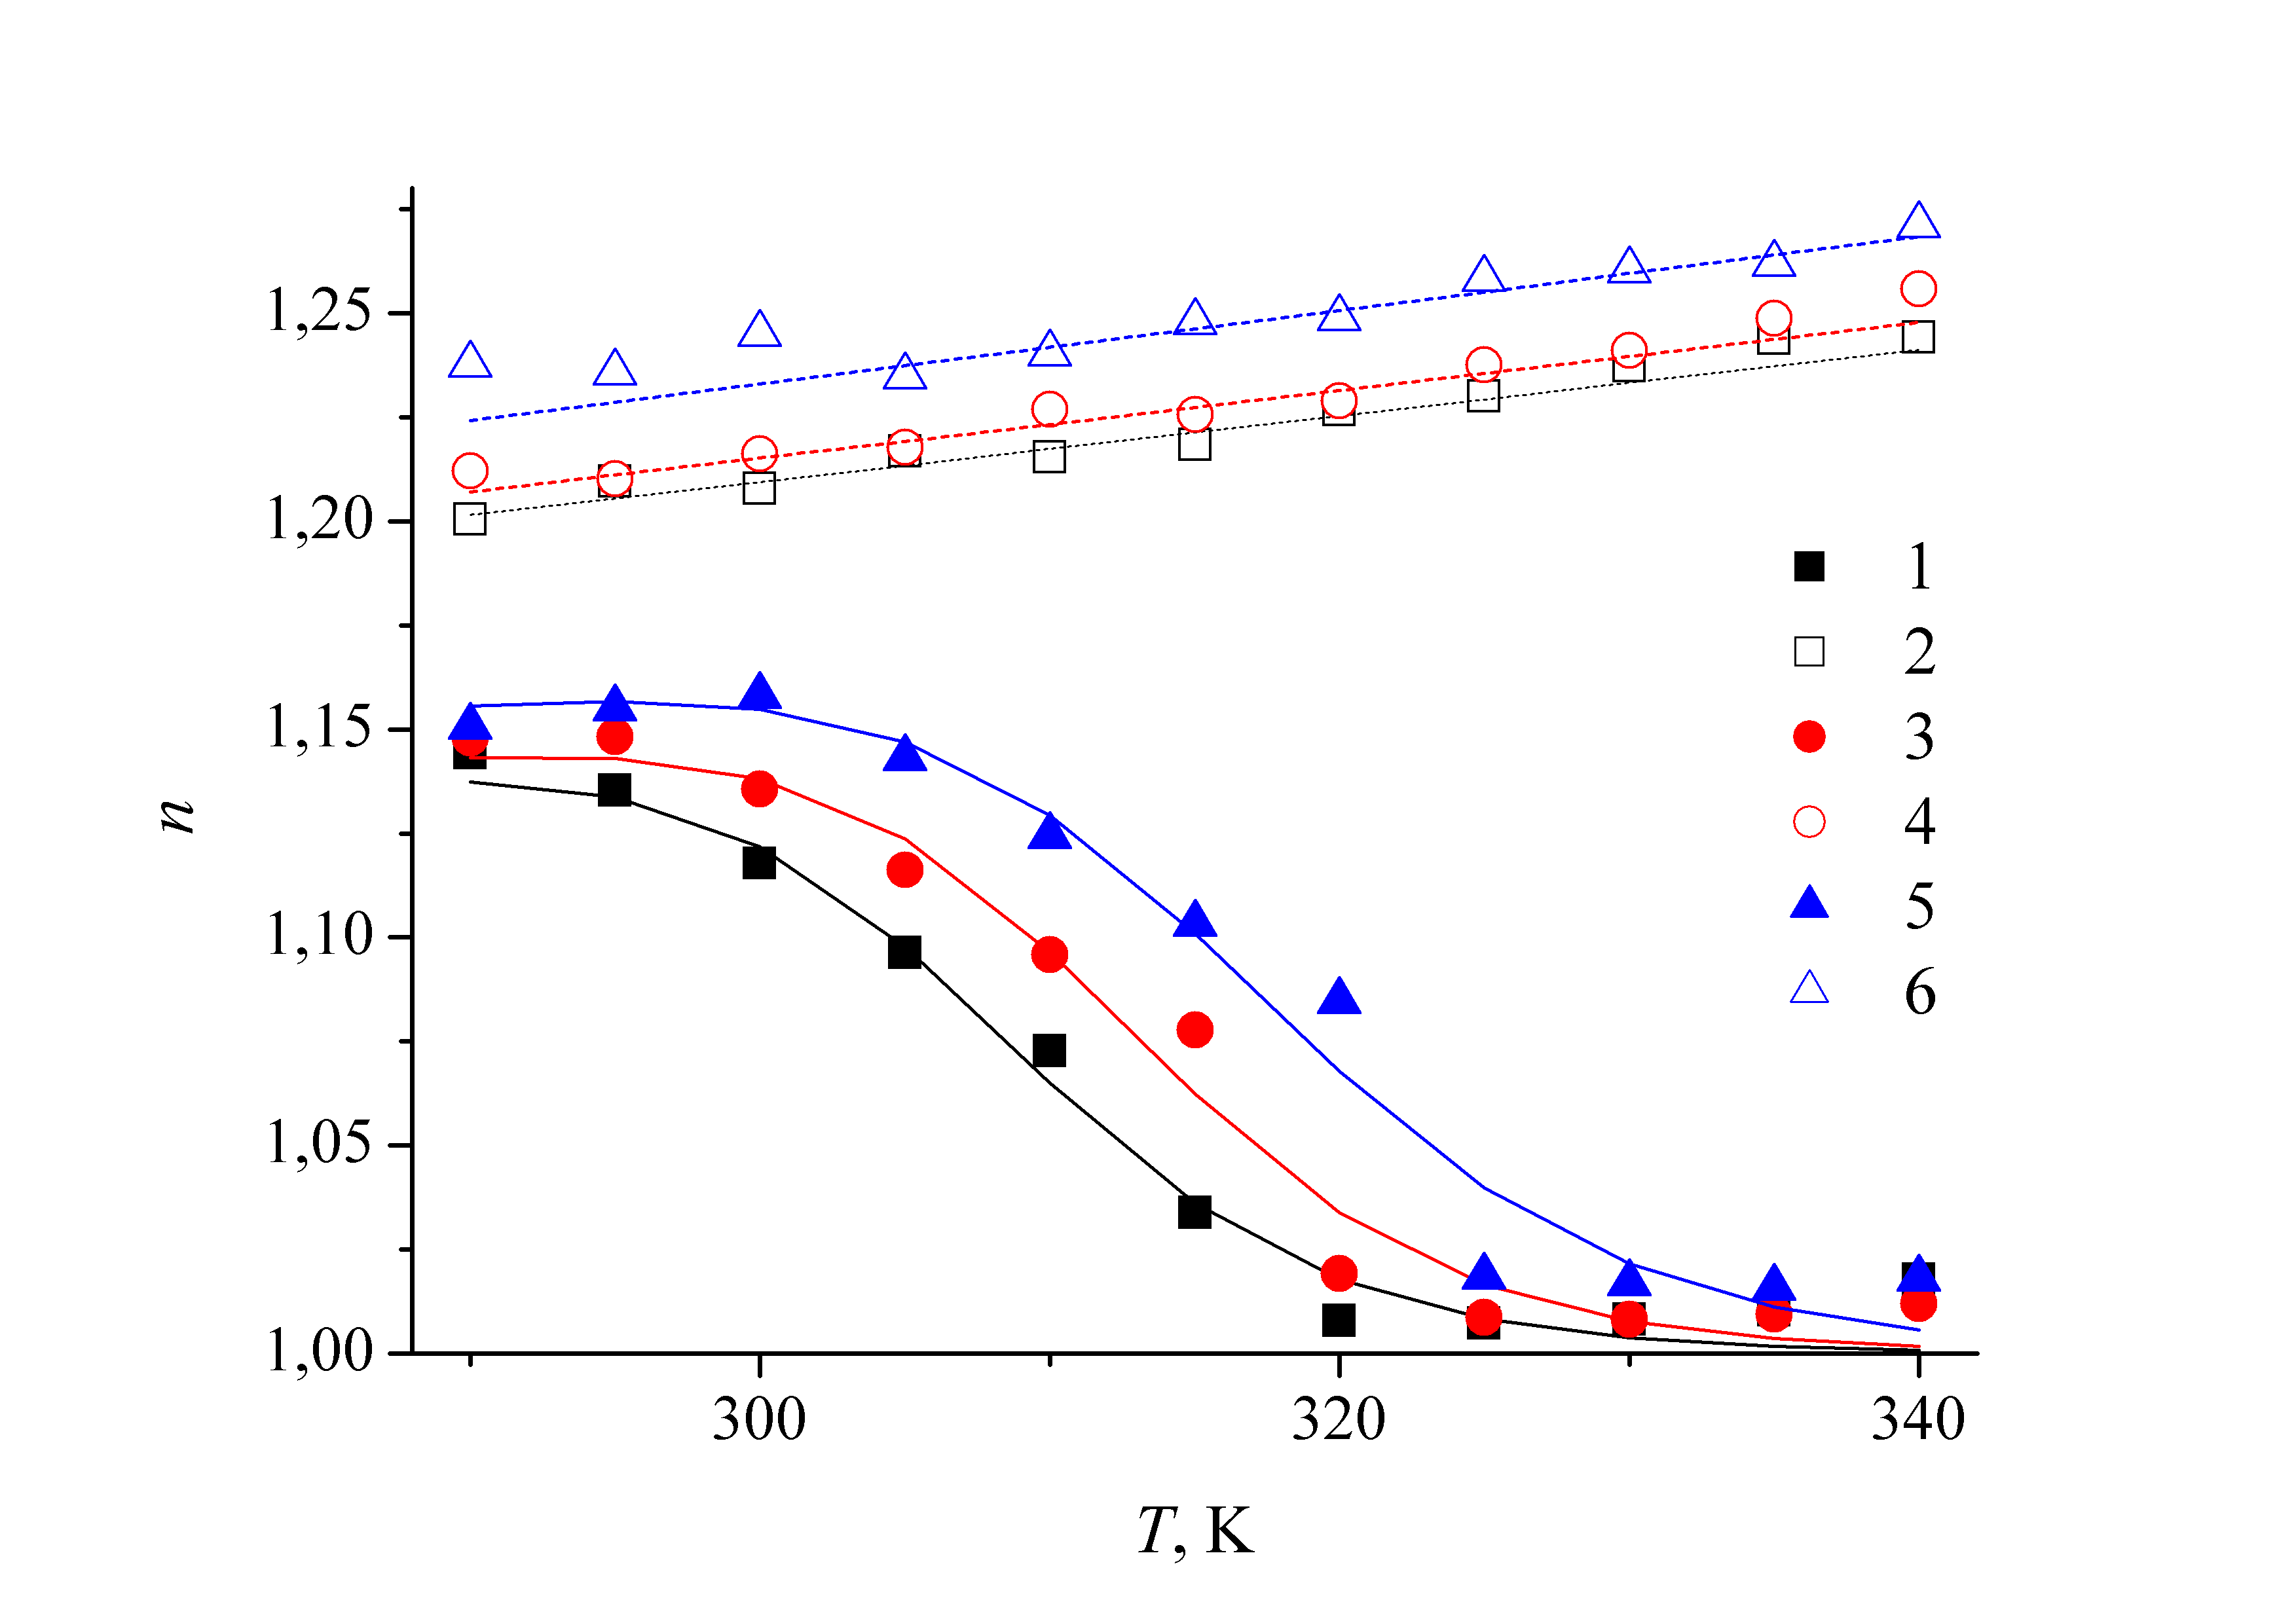
\includegraphics[width=0.85\textwidth]{Fig3_6}
\vspace{-3mm}
\caption{Розраховані доплерівські
спектри анігіляції позитронів, захоплених
вакансією (а), комплексами вакансія--сурма (б),
$\mbox{V}-\mbox{Sb}_2$ (в),
Товста лінія показує повний спектр,
тонкі --- на окремих оболонках як атому кремнію,
так і домішок.
Рисунок адаптовано з \cite{PAS}.
}
\vspace{-3mm}
\label{F36}
\end{figure}

Аналіз $(W_+-S_+)$ залежностей для різних зразків
дозволяє отримати інформацію про процеси перебудова дефектної підсистеми.
Наприклад, в $\text{In}_x\text{Ga}_{1-x}\text{N}$
процес декорування катіонної вакансії
вакансією азоту супроводжується зсувом вказаної залежності в бік
менших значень $W_+$ та більших $S_+$.



Додаткову інформацію щодо розподілу дефектів
у, наприклад, шаруватих структурах
можна отримати з аналізу залежностей параметрів
форми від енергії монохроматичних позитронів \cite{Uedono_2014}.
